\documentclass[12pt,a4paper]{article}
\usepackage[utf8]{inputenc}
\usepackage[english]{babel}
\usepackage{enumerate}
\usepackage{amsmath}
\usepackage{amsfonts}
\usepackage{amssymb}
\usepackage{graphicx}
\usepackage{fourier}
\usepackage[left=2cm,right=2cm,top=2cm,bottom=2cm]{geometry}
\usepackage{commath}
\usepackage{cancel}
\usepackage{placeins}
\author{Juan Carlos Apitz, ID 012523821}
\title{STAT572 - In Class Test 1}
\begin{document}

\maketitle

\section*{Question 1}

\textit{Part a.}

\textbf{Procedure}
For this question we first define a function handle $f(x)$ to calculate the Slash distribution per the question. Then:

\begin{enumerate}
\item{
Generate a set of uniform random values between 0 and 1, call it $u$.
}

\item{
Generate values which are necessarily between 0 and 1 from the Slash CDF, call it $F(x)$.
}

\item{
If $F(x)>u$, then we deem this $x$ value as having come from the Slash distribution and we keep it in the random sample, otherwise we discard the particular $x$ value. We do this for all values of $x$ in the domain, which for the Slash is infinite, so we choose the domain $(-5<x<5)$ which contains most of the density of the Slash distribution. This is our random sample.
}
\end{enumerate}

\textbf{Code}\\
\textit{Slash PDF}
\begin{verbatim}
function [x] = slash(y)
x = zeros(size(y));
for i = 1:length(y)
    if y(i) ~= 0
        x(i) = (1-exp(-y(i).^2/2))/((y(i).^2)*sqrt(2*pi));
    else
        x = 1/(2*sqrt(2*pi));
    end
end
\end{verbatim}

\textit{Script to Generate Data and Analysis}

\begin{verbatim}
%initialize parameters
n = 100; % sample size
M = 1000;
x=linspace(-5,5,100);
F=zeros(size(x));
rs=zeros(size(x));
u=rand(1,200);
% Monte Carlo loop
par = zeros(1,M);

% Loop thru uniforms and x vector picking x's that meet criteria
for i=1:length(u)
    for j=1:length(x)
        if quadgk(@(x)slash(x),-inf,x(j))<u(i)
            F(j)=1;
        else
            F(j)=quadgk(@(x)slash(x),-inf,x(j));
        end
    end
    if min(F) ~= 1
        l=find(F==min(F));
        rs(i)=x(l);
    end
end

% plots
figure(1)
HIST =  hist(rs);
bar(-5:1.1:5,HIST/length(u),1,'w')
title('Frequecy Histogram of Slash Random Sample')
hold on
plot(x,g);
axis([-6 6 0 0.25])
hold off

figure(2)
plot(x,y);

figure(3)
cdfplot(rs);

% Monte Carlo
M= 1000;
MUHAT= mean(rs);
SIGMAHAT= std(rs);

for i= 1:M
rsho = normrnd(1,SIGMAHAT);
trs(i)= mean(rsho);
end

alpha= 0.05;
ind= find( trs >= median(rs));
PVAL= length(ind)/M;
\end{verbatim}

\textbf{Results}

\begin{figure}[ht!]
\begin{center}
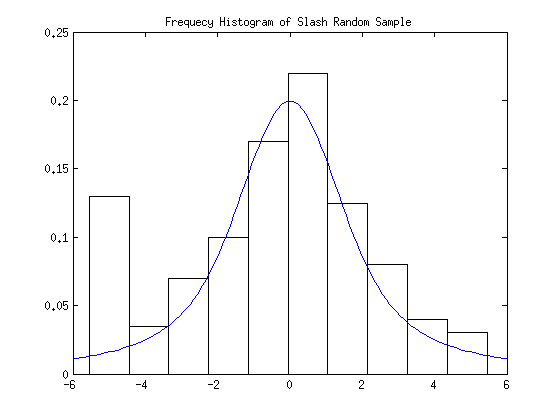
\includegraphics[scale=.9]{q1_density.png}
\caption{Density Histogram of Slash Random Sample}
\label{q1 fig1}
\end{center}
\end{figure}
\FloatBarrier

\begin{figure}[ht!]
\begin{center}
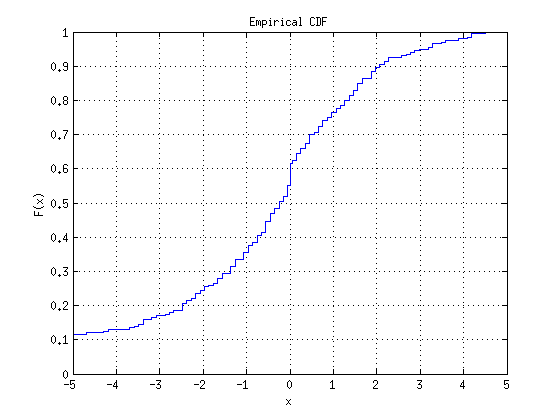
\includegraphics[scale=.9]{q1_empirical.png}
\caption{Empirical CDF Slash Random Sample}
\label{q1 fig2}
\end{center}
\end{figure}
\FloatBarrier

\begin{figure}[ht!]
\begin{center}
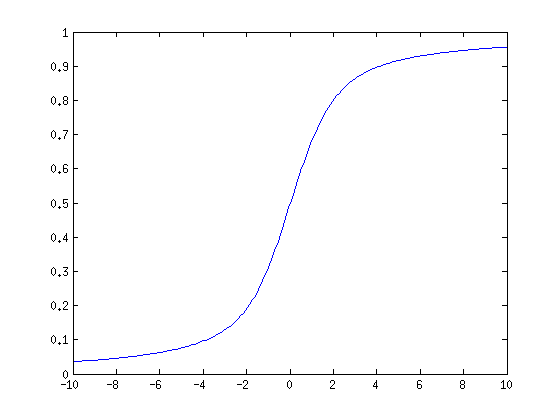
\includegraphics[scale=.9]{q1_theoretical.png}
\caption{Theoretical CDF of Slash Dist}
\label{q1 fig1}
\end{center}
\end{figure}
\FloatBarrier

As expected the, theoretical Slash CDF generated from the pdf function per the question closely resembles the cdf generated by the random sample.

\textit{Part b.}

\textbf{Procedure}
To generate a Monte Carlo simulation  to perform hypothesis testing on the population median, i.e.

\[H_o: m\leq 1\text{ vs. }H_1 > 1\]

\begin{enumerate}
\item{
Doing hypothesis testing about the median for the Slash distribution is similar to doing hypothesis testing for the mean because the Slash distribution is symmetric, just like the normal except that it has fatter tails.\\

We calculate the test statistic of from the random sample generated by the Slash of size $200$. In this case we calculate the median $m$ from the random sample generated in a).
}

\item{
Then we use the normal as a pseudo population, which is reasonable since the normal and the Slash share many characteristics. We sample from the normal under the null hypothesis, i.e. the pseudo population is $N\bigr(1,\sigma^2_{slash}\bigr)$. I set up the simulation at $M=1000$.
}

\item{
For each sample we calculate the median $m_o$, and after the Monte Carlo sampling is complete we have a vector of 1000 $m_o$, medians with an expected value of 1.
}

\item{
Then we estimate the p-value by looking at the sample of medians with expected value 1 generated by the Monte Carlo process and seeing what percent of these values are above the median of the random sample generated in a). That is we count how many of the 1000 medians generated from the simulation are greater than the median of the random sample generated in a) divide by 1000, the number of Monte Carlo simulation. We obtain a value of $65.6\%$. 
}

\item{
From the above result we conclude that the random sample does not come from a distribution that is normal with median/mean that is $>1$, we fail to reject the null hypothesis that $m\leq1$.
}


\end{enumerate}

\textbf{Code}\\
\begin{verbatim}
% Monte Carlo
M= 1000;
MUHAT= mean(rs);
SIGMAHAT= std(rs);

for i= 1:M
rsho = normrnd(1,SIGMAHAT);
trs(i)= median(rsho);
end

ind= find( trs >= median(rs));
PVAL= length(ind)/M;
\end{verbatim}

\textbf{Results}\

\begin{verbatim}

>> test

PVAL =

    0.656
\end{verbatim}

\clearpage

\section*{Question 2}

\textbf{Procedure}
To use the accept/reject method we define a function handle in MATLAB that generates values for $f(x)$ as specified in the question.

\begin{enumerate}[a.]

\item{
First generate $x$ from $f(x)$.
}

\item{

Second we generate u from unif$(2,6)=g(x)$

}

\item{

Third if $u\leq\dfrac{f(x)}{cg(x)}$
}

\end{enumerate}

The constant c is given by the max$\biggr(f(x)\biggr)=\dfrac{1}{2}$. 

\textbf{Code}\\
\textit{Function Handle}
\begin{verbatim}
function [y] = q2pdf(x)

if x<3 && x>=2
    y = (x-2)/2;
else x<=6 && x>=3;
    y = (2-(x/3))/2;
end
\end{verbatim}

\textit{Script}
\begin{verbatim}
f = @(x) q2pdf(x);
c = 0.5;
n=300;  % generate 100 rv's
% set up the arrays to store variates
x = zeros(1,n); % random variates
xy = zeros(1,n); % corresponding y values
rej = zeros(1,n); % rejected variates
rejy = zeros(1,n); % corresponding y values
irv=1;			
irej=1;
while irv <= n
   y = unifrnd(2,6);  % random number from g(y)
   u = unifrnd(2,6);  % random number for comparison
   if u <= f(y)/(0.25*c);
      x(irv)=y;
      xy(irv) = u*c;
      irv=irv+1;
   else
      rej(irej)= y;
      rejy(irej) = u*c; % really comparing u*c<=2*y
      irej = irej + 1;
   end
end
figure(1)
plot(x,xy,'o',rej,rejy,'*')
axis square %([0 1 0 c])
title('Accepted/Rejected')

figure(2)
[fr,x]=hist(x);
h=x(2)-x(1);
bar(x,fr/(n*h),1,'w')
title('Frequency Histogram of Random Sample')
hold on

x = linspace(2,6);
y = zeros(size(x));
for i = 1:length(x)
    y(i) = q2pdf(x(i));
end
plot(x,y);

probrej = irej/(irej+n);
\end{verbatim}

\textbf{Output}\\

\begin{figure}[ht!]
\begin{center}
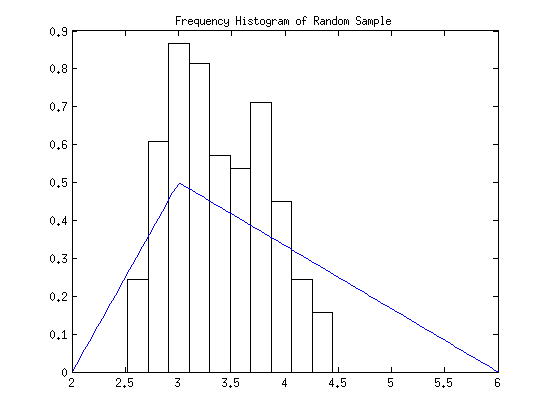
\includegraphics[scale=.9]{q2_hist.png}
\caption{Accept/Reject Histogram}
\label{q2 fig1}
\end{center}
\end{figure}
\FloatBarrier

\begin{figure}[ht!]
\begin{center}
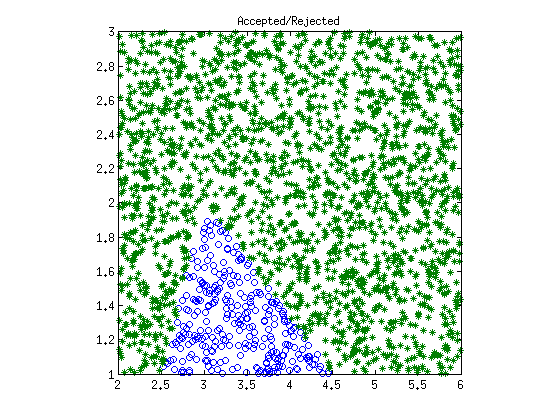
\includegraphics[scale=.9]{q2_graph.png}
\caption{Accept/Reject}
\label{q2 fig2}
\end{center}
\end{figure}
\FloatBarrier

\textit{Probability of rejection:}
\begin{verbatim}
>> probrej

probrej =

    0.8754
\end{verbatim}

\clearpage

\section*{Question 3}

\textbf{Procedure}\\

\begin{enumerate}
\item{
Calculate the $\theta$ value using the quad function to get an approximately exact value.
}

\item{

Use Monte Carlo simulations with $M=100$ to estimate the MSE of the first estimate $\hat{\theta_1}$ and the second estimate $\hat{\theta_2}$.
}

\item{
Compare the MSEs. The smallest one is the best estimate.
}
\end{enumerate}

\textbf{Code}\\

\begin{verbatim}
theta = quad('exp(x.^2)',0,1);
MSE1 = zeros(1,100);
MSE2 = zeros(1,100);
for i = 1:100
    u = unifrnd(0,1,1);
    u1 = unifrnd(0,1,1);
    u2 = unifrnd(0,1,1);
    thetahat1 = (1/2)*exp(u.^2)*(1+exp(1-2*u));
    thetahat2 = (1/2)*(exp(u1.^2)+exp(u2.^2));
    MSE1(i) = abs(theta - thetahat1)^2;
    MSE2(i) = abs(theta - thetahat2)^2;
end
MSE1 = mean(MSE1);
MSE2 = mean(MSE2);
\end{verbatim}

\textbf{Results}\\
The results show that the first estimate procedure is better because it produces an MSE of 0.0230 vs 0.1431. So we can argue that the first estimate is better. 

\begin{verbatim}
>> MSE1

MSE1 =

    0.0230

>> MSE2

MSE2 =

    0.1431
\end{verbatim}
\clearpage

\section*{Question 4}

\textbf{Procedure}

We can use the bootstrap approach by estimating the population mean because \[P\biggr(a<\dfrac{\bar{X}-\mu}{SE(\bar{x}}<b\biggr)=P\biggr(\bar{X}-aSE(\bar{x})>\mu>\bar{X}-bSE(\bar{x})\biggr)\]
So we can estimate $P$ by finding an interval for $\mu$ and estimating its coverage. We can do this repeatedly and generate a series of coverage estimates, and use the mean of all these coverage estimates as $\hat{P}$. Then a $(1-\alpha)CI$ can be constructed as $\biggr(\hat{P}-z_{1-\alpha/2}SE(\hat{P}),\hat{P}-z_{\alpha/2}SE(\hat{P})\biggr)$

\textbf{Code}\\
\begin{verbatim}
% STANDARD BOOTSTRAP CI
load forearm
counter = 0; B = 500; counterv = zeros(1,50);
meand = mean(forearm); stdev = std(forearm);
thetahatb = zeros(1,100);
for k = 1:50
    for i=1:100
        % generate data and calculate stat of interest
        rs = normrnd(meand,stdev,1,20);
        thetahat = mean(rs);
        
        % set up the Bootstrap
        bvals = bootstrp(B, @(x) mean(x),rs);
        
        % calculate the Bootstrap SE
        seb = std(bvals);
        
        % calculate the CI
        alpha = 0.05;
        cilo = thetahat-(2)*seb;
        cihi = thetahat-(-2)*seb;
        if cihi >= meand && cilo <= meand
            counter = counter + 1;
        end
        thetahatb(i) = mean(bvals);
    end
    counterv(k) = counter;
    counter = 0;
end
pmean = mean(counterv);
pse = std(counterv)/sqrt(k);
alpha = 0.05;
ciplo = pmean-norminv(1-alpha/2,0,1)*pse;
ciphi = pmean-norminv(alpha/2,0,1)*pse;
\end{verbatim}

\textbf{Results}\

\begin{verbatim}
>> ciphi

ciphi =

   93.4155

>> ciplo

ciplo =

   91.8645
\end{verbatim}

\textbf{Discussion}\\
The above result shows that our interval is $(91.8645, 93.4155)$ which is not really a good interval. The expectation is that this interval should contain 95 percent, which is closer to the true value of P.
\end{document}
